\subsection{The Evolving Role of the Draft Sequence}
\label{sec:draft-background}

A shutter event produces multiple image buffers. The full post-processing path
collects the required buffers, performs multi-frame composition and image
enhancement, encodes the result, and stores the final image file. The Draft
Sequence was introduced together with this pipeline to provide a capture result
quickly while final processing continues. It also retains the Draft image as a
recovery result if final processing fails. The Draft is therefore both a
user-visible capture result and a reliability mechanism, rather than an
internal preview artifact. Showing the captured image to the user quickly and
keeping the Draft visually consistent with the final image are consequently
important to camera usability.

As final post-processing became more sophisticated, it required greater compute
and memory resources and produced larger visual changes, widening the gap
between untreated Draft and final images. Executing this processing immediately
after capture can also interfere with foreground camera operation, causing
dropped preview frames and less responsive interaction. Selected capture modes
therefore defer full composition until the camera application switches to the
background. This deferral keeps the Draft image visible to the user for longer,
making missing effects more noticeable and increasing the need for Draft--final
consistency. Figure~\ref{fig:draft-pipeline} illustrates this structure.

Initially, the Draft was produced by encoding the selected input without
applying image effects. Filter and Watermark were the first effects added to the
Draft Sequence, using single-frame processing to narrow the visible difference
between Draft and final images. As post-processing increasingly adopts AI-based
algorithms, the resulting visual changes can no longer be reproduced adequately
by the Draft Sequence's existing single-frame stages. Portrait capture has the
largest Draft--final visual gap because its final processing combines
multi-frame composition with Bokeh. Its Draft Sequence therefore requires
lightweight multi-frame Draft Bokeh to make the user-visible Draft more
representative of the final portrait.

% Companion draft and final paths in the camera post-processing pipeline.
% Included from _2_preliminary.tex.
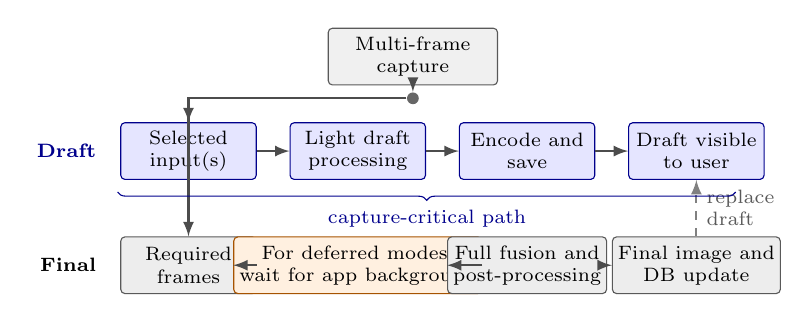
\begin{tikzpicture}[
  font=\scriptsize,
  >=latex,
  box/.style={draw=black!65, rounded corners=1.5pt, align=center,
    minimum width=1.72cm, minimum height=0.72cm, inner sep=2pt},
  draft/.style={box, draw=blue!55!black, fill=blue!10},
  final/.style={box, draw=black!65, fill=gray!14},
  gate/.style={box, draw=orange!65!black, fill=orange!12},
  flow/.style={->, thick, black!70},
  split/.style={circle, fill=black!60, inner sep=1.5pt}
]

  \node[box, fill=black!6, minimum width=2.15cm] (capture) at (3.85,3.55)
    {Multi-frame\\capture};
  \node[split] (fork) at (3.85,3.02) {};
  \draw[flow] (capture) -- (fork);

  % Draft lane.
  \node[anchor=east, font=\scriptsize\bfseries, text=blue!55!black]
    at (-0.05,2.35) {Draft};
  \node[draft] (dinput) at (1.00,2.35) {Selected\\input(s)};
  \node[draft] (deffect) at (3.15,2.35) {Light draft\\processing};
  \node[draft] (dsave) at (5.30,2.35) {Encode and\\save};
  \node[draft] (dvisible) at (7.45,2.35) {Draft visible\\to user};

  \draw[flow] (fork) -| (dinput.north);
  \draw[flow] (dinput) -- (deffect);
  \draw[flow] (deffect) -- (dsave);
  \draw[flow] (dsave) -- (dvisible);

  % Final lane.
  \node[anchor=east, font=\scriptsize\bfseries] at (-0.05,0.90) {Final};
  \node[final] (finput) at (1.00,0.90) {Required\\frames};
  \node[gate] (fgate) at (3.15,0.90) {For deferred modes:\\wait for app background};
  \node[final] (fprocess) at (5.30,0.90) {Full fusion and\\post-processing};
  \node[final] (fupdate) at (7.45,0.90) {Final image and\\DB update};

  \draw[flow] (fork) -| (finput.north);
  \draw[flow] (finput) -- (fgate);
  \draw[flow] (fgate) -- (fprocess);
  \draw[flow] (fprocess) -- (fupdate);

  % The final result replaces the published draft entry.
  \draw[flow, dashed, black!50] (fupdate.north) -- (dvisible.south)
    node[midway, right, align=left, text=black!65] {replace\\draft};

  \draw[decorate, decoration={brace, mirror, amplitude=3pt}, blue!55!black]
    (0.10,1.83) -- (7.95,1.83);
  \node[anchor=north, text=blue!55!black] at (4.03,1.72)
    {capture-critical path};

\end{tikzpicture}
